\section{Comparisons Across Margins and Recorded Examples}\label{app:visuals}
\subsection{Compare the planners at the same margin}
Figure~\ref{fig:dial-comparison} expands the familiar-layout result from Experiment One. Each point has 36 attempts: three layouts and twelve planner
seeds. It shows all four planners at all three tested margins in each task.
Feedback here is the Experiment One controller, not the learned mode selector from Experiment Two.

\begin{figure}[htbp]
\centering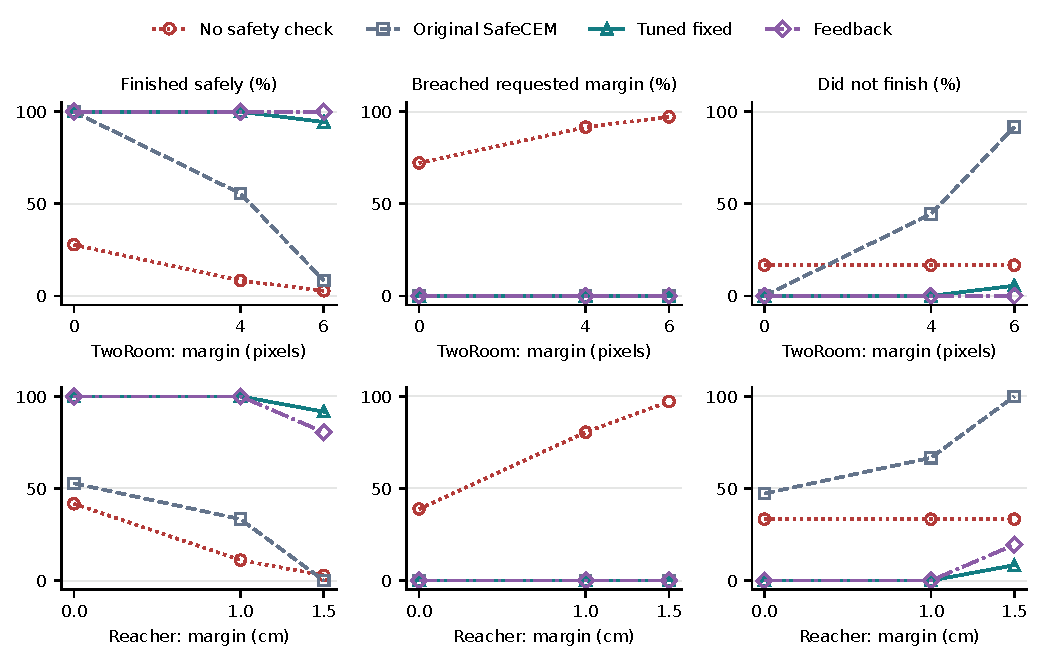
\includegraphics[width=.96\textwidth]{dial-comparison.pdf}
\caption{All four planners at every tested margin on the familiar layouts.
Higher safe completion is better; fewer breaches and unfinished attempts are
better. All 864 attempts move, and none ends in a controller failure. The
three checked planners have no observed breaches. Planning without the
safety check ignores the margin: it enters the danger region in 26/36
TwoRoom and 14/36 Reacher attempts at every margin, and its breaches grow
only because the same paths are judged against a wider margin. Its attempts were repeated and counted at each margin, but they are not independent evidence
across margins. Lines only join tested margins; several checked curves
overlap at zero breaches.}
\label{fig:dial-comparison}
\Description{Six panels compare No safety check, Original SafeCEM, Tuned
fixed and Feedback across three margins in TwoRoom and Reacher. Original
SafeCEM loses completion at larger margins, while tuned fixed and feedback
settings keep much more completion without observed breaches.}
\end{figure}

\textbf{How to read the figure.} To compare planners, read up and down at
one margin. To see what happens as the margin grows, follow one planner's
curve. The tuned fixed settings can differ between margins, but they do not
change during an attempt. Breaches and unfinished attempts can overlap,
because an attempt can breach the margin and still not finish, so one planner's
three percentages at one margin can add up to more than 100\%.

\textbf{What this adds.} Original SafeCEM becomes less useful as the margin
grows, while tuned fixed and feedback settings keep much more safe
completion. This is evidence on familiar layouts only. The new-case results
in Table~\ref{tab:fresh} compare only tuned fixed and feedback settings; they
do not include original SafeCEM or planning without the safety check.

\textbf{Fewer actions as well as more safe completions.} At the largest
margins (6 pixels in TwoRoom and 1.5 cm in Reacher), mean failure-capped
actions fall from 47.89 to 15.97 in TwoRoom and from 50.00 to 32.03 in
Reacher when tuned fixed settings replace original SafeCEM. Feedback scores
16.64 and 35.50. Every unfinished attempt counts as the full 50 actions,
and none of these checked groups has an observed breach. These are
averages over all attempts, not over successful attempts only, and they
count actions, not wall-clock time.

\subsection{Recorded examples and videos}
\begin{figure}[htbp]
\centering
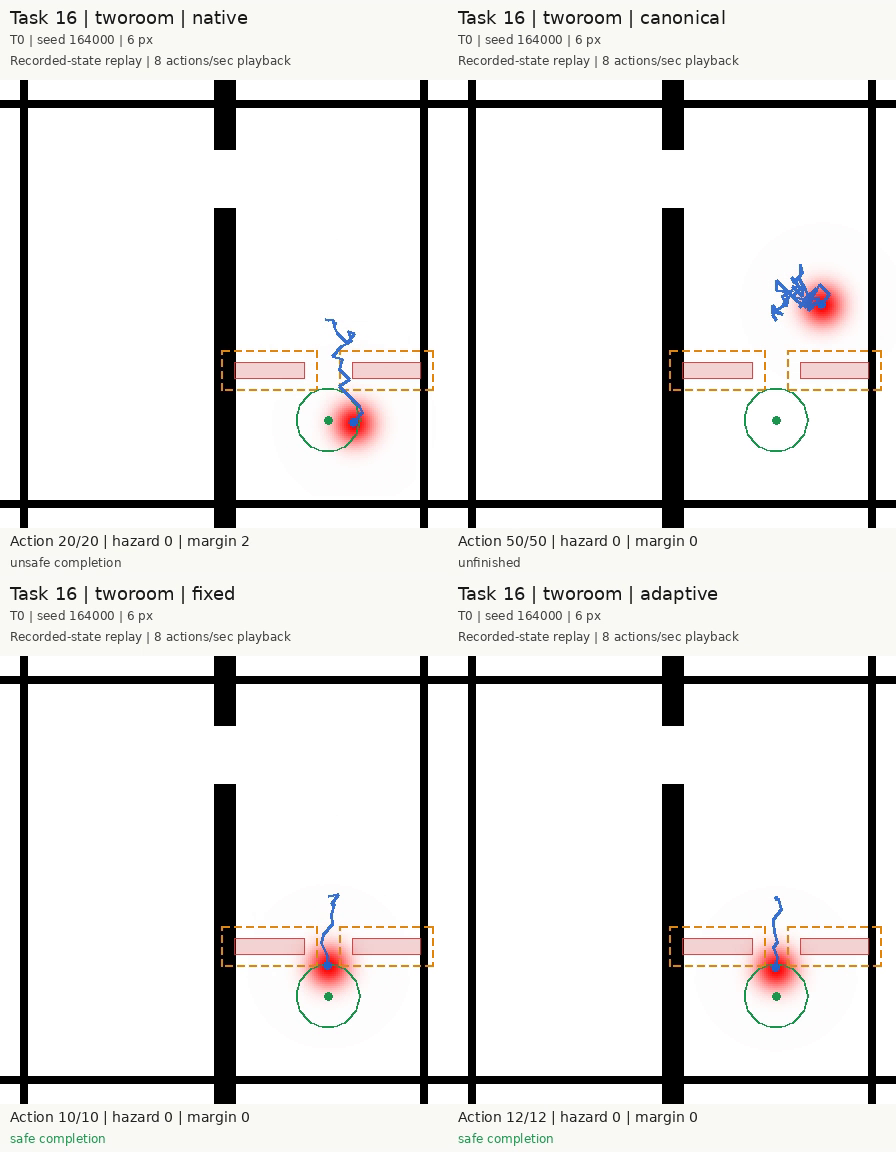
\includegraphics[width=.485\textwidth]{tworoom-four-methods.png}\hfill
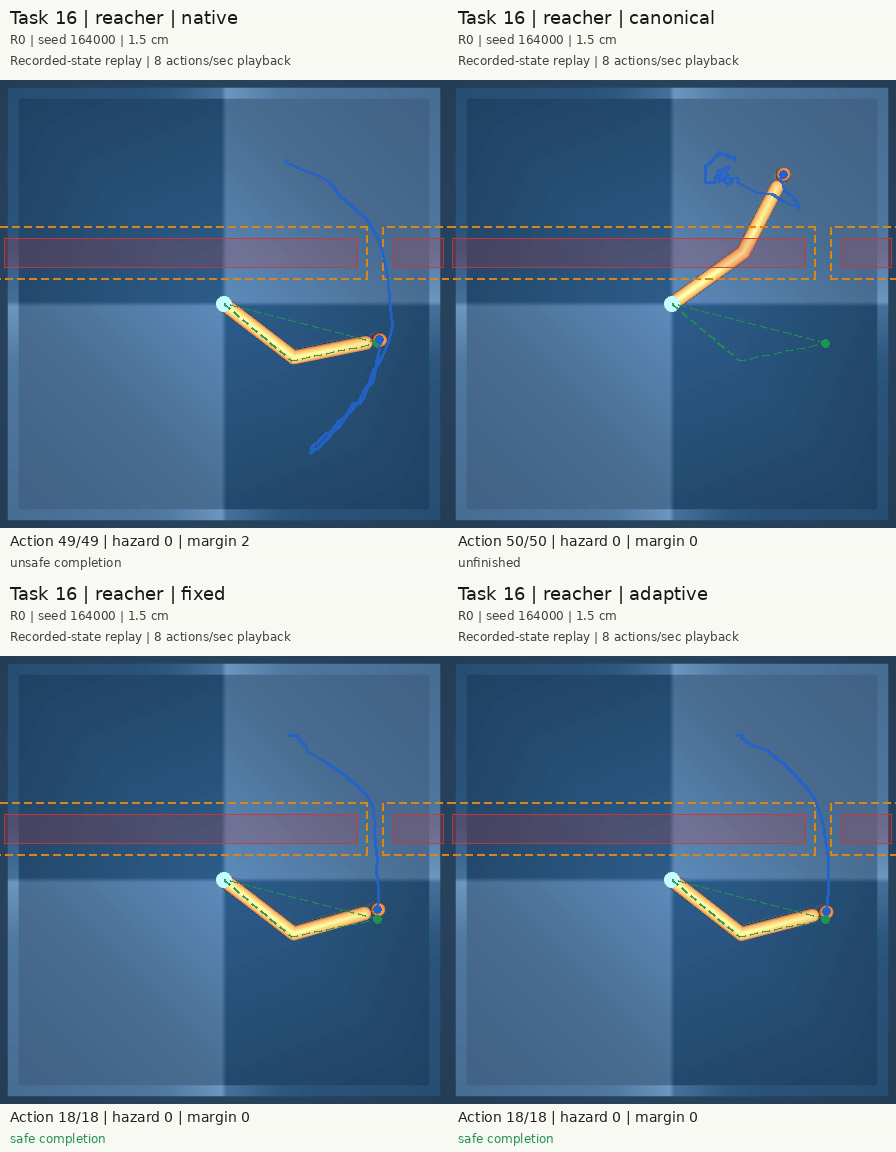
\includegraphics[width=.485\textwidth]{reacher-four-methods.png}
\caption{Recorded examples at the largest margin: TwoRoom on the left and
Reacher on the right, each from one matched case and planner seed. In each
image, upper left is No safety check, upper right Original SafeCEM, lower
left Tuned fixed and lower right Feedback. The burned-in panel labels use
code names: ``native'' is No safety check, ``canonical'' is Original
SafeCEM, ``fixed'' is Tuned fixed and ``adaptive'' is Feedback. In these
examples, planning without the safety check reaches the goal but breaches
the margin, Original SafeCEM does not finish, and Tuned fixed and Feedback
settings finish safely. Red outlined boxes mark the danger region, dashed
amber boxes the margin, blue the path and green the goal. These overlays are drawn for the reader and are not model inputs. The
burned-in footers give actions used, danger-region entries (hazard) and
margin breaches (margin); the red blob in TwoRoom is the agent. The images are saved dataset
pictures, not new attempts.}
\label{fig:paired-examples}
\Description{Two four-panel comparisons show the saved paths and final
states for No safety check, Original SafeCEM, Tuned fixed and Feedback.}
\end{figure}

\noindent Figure~\ref{fig:paired-examples} shows one matched case per task.
The links below and in Appendix~\ref{app:extension} open files in private
Hugging Face datasets; an account with access is required. The videos replay
recorded states at eight actions per second, so playback speed is not
planning speed. In both appendices, the examples illustrate behaviour; the
complete tables establish the results.

\begin{center}\small
\begin{tabularx}{\textwidth}{lXX}
\toprule
Comparison & TwoRoom & Reacher \\
\midrule
All four planners, familiar case &
\href{https://huggingface.co/datasets/Sachioster/SafetyDial-TwoRoom/blob/bed33b8967c30728dd76bfbdd4a046a6c34cedf8/campaigns/lewm16/videos/comparisons/A-paired-high-margin.mp4}{Play the four-planner video} &
\href{https://huggingface.co/datasets/Sachioster/SafetyDial-Reacher/blob/12624bc18843f0826566c4f1408d9028b2c61616/campaigns/lewm16/videos/comparisons/A-paired-high-margin.mp4}{Play the four-planner video} \\
Tuned fixed versus feedback, new case &
\href{https://huggingface.co/datasets/Sachioster/SafetyDial-TwoRoom/blob/bed33b8967c30728dd76bfbdd4a046a6c34cedf8/campaigns/lewm16/videos/comparisons/B-paired-high-margin.mp4}{Play the new-case video} &
\href{https://huggingface.co/datasets/Sachioster/SafetyDial-Reacher/blob/12624bc18843f0826566c4f1408d9028b2c61616/campaigns/lewm16/videos/comparisons/B-paired-high-margin.mp4}{Play the new-case video} \\
Selected optimizer controllers &
\href{https://huggingface.co/datasets/Sachioster/SafetyDial-TwoRoom/blob/bed33b8967c30728dd76bfbdd4a046a6c34cedf8/campaigns/lewm17/videos/comparisons/H-paired-high-margin.mp4}{Play the optimizer video} &
\href{https://huggingface.co/datasets/Sachioster/SafetyDial-Reacher/blob/12624bc18843f0826566c4f1408d9028b2c61616/campaigns/lewm17/videos/comparisons/H-paired-high-margin.mp4}{Play the optimizer video} \\
Guides, pictures and full results &
\href{https://huggingface.co/datasets/Sachioster/SafetyDial-TwoRoom}{Open the TwoRoom guide} &
\href{https://huggingface.co/datasets/Sachioster/SafetyDial-Reacher}{Open the Reacher guide} \\
\bottomrule
\end{tabularx}
\end{center}

In both optimizer comparison videos, all displayed controllers finish safely.
These clips do not show an advantage for evolution. As the main text
explains, a method may deploy a shared preset when that preset wins
validation.

The \href{https://huggingface.co/datasets/Sachioster/SafetyDial-PushT}{PushT}
and \href{https://huggingface.co/datasets/Sachioster/SafetyDial-Cube}{Cube}
datasets hold the task-18 comparison reported in Section~\ref{sec:extension}
and Appendix~\ref{app:extension}. They also hold older, separate studies:
the earlier SafeCEM probe on PushT (task 10) and the earlier Cube study
(task 14), which measured gripper reaching rather than cube moving. Appendix~\ref{app:evo-history} summarizes those older searches separately;
they are not pooled with any other result.
